\chapter{Entorno de Simulación y Objeto de Estudio}

\section{1200 V CoolSiC MOSFET}

Growing environmental concerns and global energy regulations are accelerating the transition to energy-efficient motor drive systems. There is increasing demand for compact, high-efficiency, and reliable inverters across HVAC, industrial, and automation sectors. 

\cite{11269412}



Infineon Technologies introduced 1200 V CoolSiC MOSFET technology in 2017. In comparison to traditional silicon (Si) based high voltage (> 600V) switches like IGBTs and MOSFETs, the SiC MOSFET offers a series of advantages. These include the lowest gate charge and device capacitance levels seen in 1200 V switches, less reverse recovery losses of the body diode, temperature-independent low switching losses, and threshold-free on-state characteristics. 

\begin{figure}  
    \label{figure: Esquema MOSFET}
    \centering
    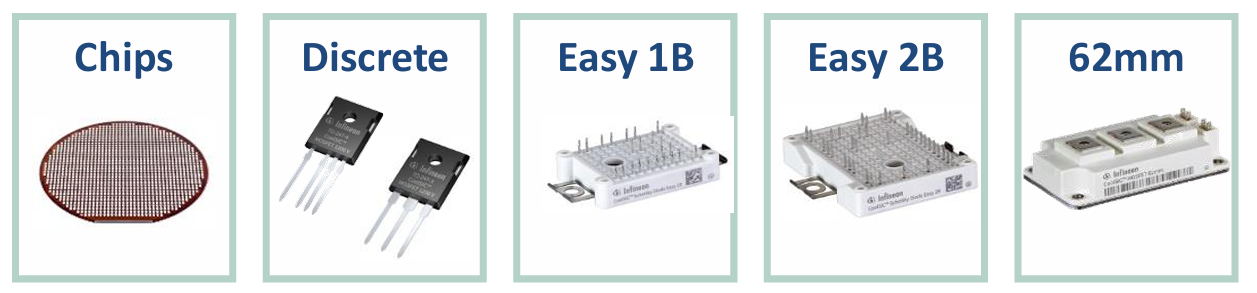
\includegraphics[width = 0.75  \textwidth]{Imagenes/Solutions using 1200 V CoolSiC MOSFET.png}
    \caption{Soluciones con MOSFET CoolSiC de 1200 V \cite{infineonAN2017-46}}
\end{figure}

The new 1200 V CoolSiC MOSFET integrated in the CIPOS Maxi IPM is based on Infineon's first generation trench-type SiC MOSFET structure. Unlinke planar SiC MOSFETs, the trench architecture offers a vertical channel formation that enhances current density and reduces on-resistance per unit area.

\section{Especificaciones y parámetros del Módulo IM828-XCC}



\section{Software de simulación: Simulink}
